\documentclass{article}
\renewcommand{\thesection}{\Roman{section}}
\renewcommand{\thesubsection}{\thesection.\roman{subsection}}
\usepackage[left=0.5in, right=0.5in, top = 0.7in]{geometry}
\usepackage[utf8]{inputenc}
\usepackage[english]{babel}
\usepackage{fancyhdr}
\usepackage[dvipsnames]{xcolor}
\usepackage{graphicx}
\graphicspath{ {./images/} }
\usepackage{helvet}
\renewcommand{\familydefault}{\sfdefault}
\usepackage[export]{adjustbox}
\setlength{\parindent}{4em}
\setlength{\parskip}{1em}
\renewcommand{\baselinestretch}{1.3}
\usepackage{hyperref}
\usepackage{listings}

\pagestyle{fancy}
\fancyhf{}
\rfoot{Page \hspace{1pt} $|$ \hspace{1pt} \thepage}
\renewcommand{\headrulewidth}{0pt}
\rhead{\textcolor{CadetBlue}{Département de génie des systèmes $|$ GPA788}}

\begin{document}

\begin{minipage}{0.4\textwidth}

\includegraphics{ETS_Logo}\\
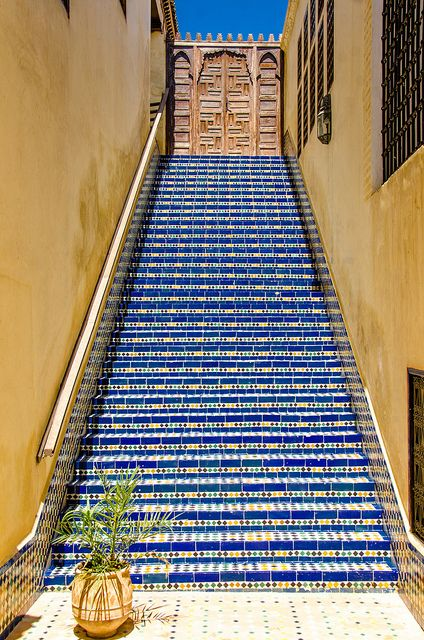
\includegraphics[width=9.5cm, height=12cm]{Intro_breather}
\bigbreak
\Huge{\textbf{\begin{flushright}{GitHub}\end{flushright}}}
\end{minipage}%
\hfill
\begin{minipage}{0.4\textwidth}
\begin{tabular}{|p{\textwidth}}
\\\\\\\\\\\\\\\\\\\\
\Large{\textcolor{Tan}{SOMMAIRE}}\\
De nos jours, le travail collaboratif à distance est une modalité de plus en plus répandue, que ce soit par nécessité ou par avantage logistique et économique. Il devient donc hautement pertinent d'être familier avec les outils populaires axés sur le développement de projet en équipe. À la tête de ces outils, sont les services Git/GitHub; Un système de gestion de versions et un serveur d'hébergement.\\\\
\Large{\textcolor{Tan}{GPA788}} \\
\textcolor{CadetBlue}{Conception et intégration de objets connectés Génie de la production automatisée}
\\\\\\\\\\\\\\\\\\\\\\\\
\end{tabular}
\end{minipage}%

\newpage
\

\newpage

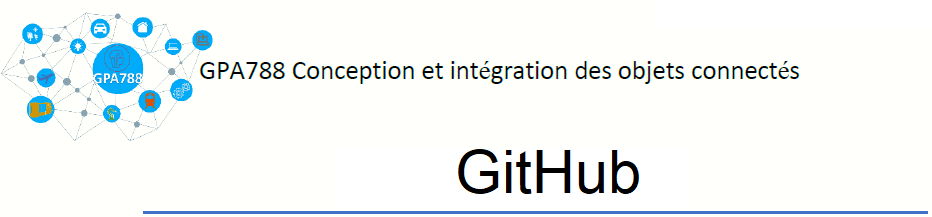
\includegraphics[width=0.75\textwidth, left]{Header}

\begin{flushleft}
    \begin{Large}{\textcolor{RoyalBlue}{Contexte}}\end{Large}\\
    L'établissement d'une connexion entre des objets et la nature de leur comportement sont deux tâches exprimées programmatiquement par une équipe de développeurs. L'ampleur d'un projet et la distance entre ses développeurs requièrent une méthodologie de travail apte à assurer une progression efficiente en équipe. À fin de réalisation de ce but, un standard autant populaire en industrie que dans le monde du \textit{open-source} est le service web d'hébergement et de gestion de développement de logiciels: GitHub. GitHub utilise le logiciel de gestion de versions Git.
\end{flushleft}

\begin{flushleft}
\begin{Large}{\textcolor{RoyalBlue}{Objectifs}}\end{Large}\\
À la fin de cette présentation, l’étudiant(e) sera capable de :
\begin{itemize}
  \item Comprendre l'utilité de GitHub
  \item Héberger son projet de développement sur GitHub
  \item Utiliser GitHub pour collaborer en équipe sur un projet de développement
\end{itemize}

\end{flushleft}

\begin{flushleft}
\begin{large}{\textcolor{RoyalBlue}{Version}}\end{large}\\
Juin 2020
\end{flushleft}

\begin{flushleft}
\begin{large}{\textcolor{RoyalBlue}{Auteur}}\end{large}\\
Ahmed Moubtahij
\end{flushleft}

\newpage
\renewcommand*\contentsname{Table des matières}
\tableofcontents

\newpage

\includegraphics[width=0.77\textwidth, center]{Github_Logo}
\begin{center}\section{Présentation d'un projet}\end{center}

\begin{flushleft}
Soit un nouveau projet ou un projet en développement tel que:\newline
\end{flushleft}

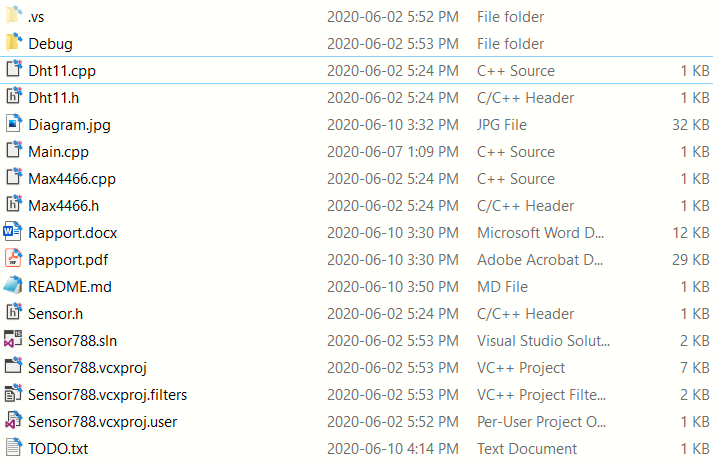
\includegraphics[width=0.65\textwidth, center]{Project_presentation}

\begin{flushleft}
On voit que le projet contient divers types de fichiers; des fichiers textes (\textit{*.txt, *.cpp, *.h, *.md}...), un fichier \textit{.pdf}, un fichier word \textit{.docx}, un fichier image \textit{.jpg}, ainsi que des dossiers et des fichiers utilitaires à Visual Studio (\textit{.vs/, Debug/, *.vcxproj, *.vcxproj.filters}). Ces fichiers résident sur notre machine, et on se réfère à leur localisation par le terme "\textbf{dépôt local}".\newline

On aimerait utiliser un serveur web pour héberger notre projet dans un \textbf{dépôt distant}. On aimerait avoir la possibilité de synchroniser la progression de notre dépôt local avec celle du dépôt distant. On aimerait décentraliser notre projet pour pouvoir l'importer à son état le plus récent vers n'importe quelle machine où on travaille, et que nos collaborateurs et lecteurs puissent en faire autant.
\end{flushleft}

\begin{center}\section{GitHub}\end{center}
\subsection{Présentation}

GitHub est un service d'hébergement de contrôle de version de développement logiciel.\\\\
Lors d'un projet, naturellement le code évolue avec le temps et de nouvelles révisions sont produites. Un système de contrôle de version (c.f. Section 4) traque ces révisions et garde les modifications dans un dépôt central. Ceci facilite grandement la collaboration, puisqu'à chaque nouvelle version du code, le développeur peut enregistrer et publier son travail sur le dépôt, et ses collaborateurs restent à jour sur la progression du projet. Ils peuvent également contribuer à sa révision et publier la dernière version sur le dépôt.\\\\
Si le dépôt est publique, des personnes autres que les collaborateurs auront accès au projet en lecture seulement, mais pourront quand même faire des requêtes de modification du code, à approuver ou refuser par le chef du projet ou ses collaborateurs en ayant le droit. Toute personne intéressée peut donc contribuer et apporter son expertise à l'évolution du projet. Ceci marque notamment la grande puissance du développement open-source.

\subsubsection{Dépôt - \textit{repository}}
Le dépôt est l'endroit où tous les fichiers d'un projet donné sont stockés, accessible avec une adresse URL unique.\\\\
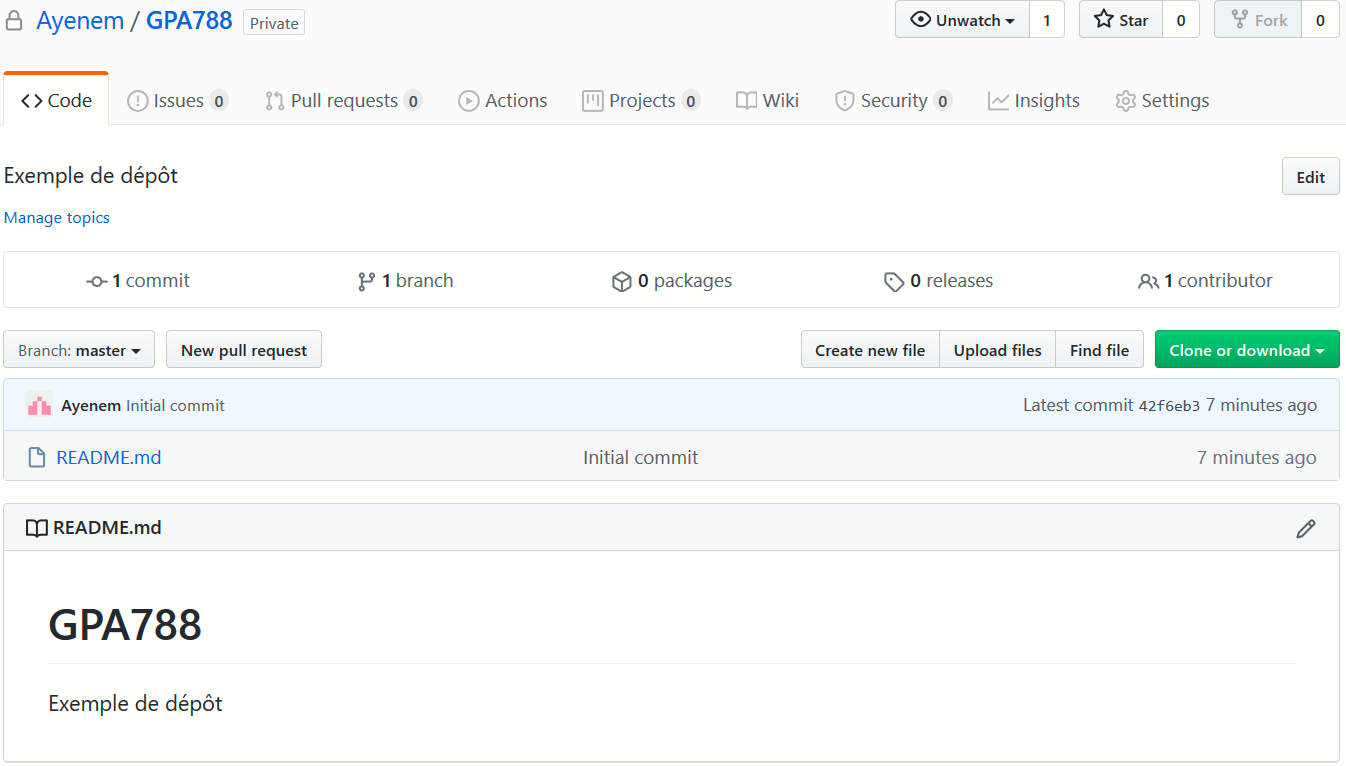
\includegraphics[width=1\textwidth, center]{Repo}
\begin{itemize}
  \item \textbf{Compte utilisateur:} Ayenem
  \item \textbf{Nom du dépôt:} GPA788
  \item \textbf{Fichiers stockés:} README.md
\end{itemize}
Le fichier \textbf{README.md} contient généralement la description du projet, ici "Exemple de dépôt".
C'est un fichier texte en format markdown, utilisé par GitHub pour que la description du projet soit directement visible sur la page du dépôt.

\subsubsection{Journal des modifications - \textit{Commits}}
GitHub traque toutes les révisions publiées sur le dépôt. Cela signifie que l'information sur "qui a changé quoi, quand, et dans quel fichier" est toujours disponible.\\\\
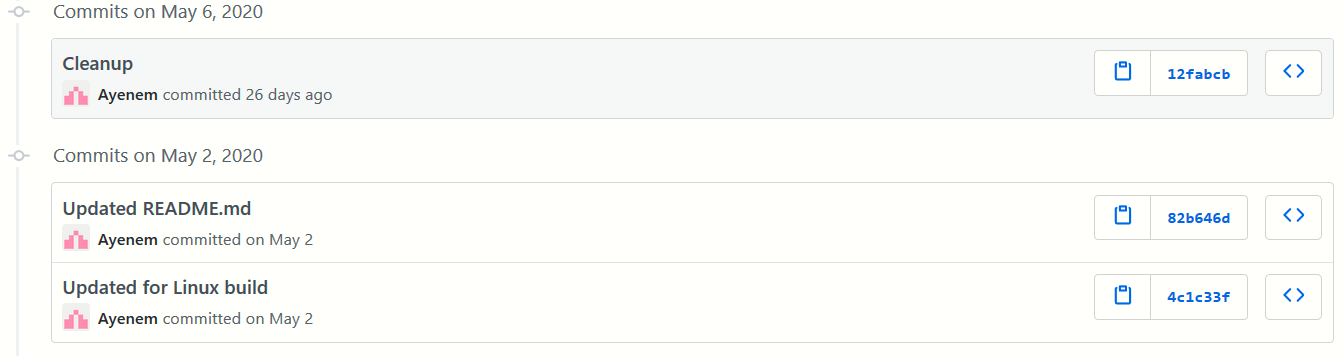
\includegraphics[width=1\textwidth, center]{ChangeLog}
En cliquant sur l'identifiant du \textit{commit} "Updated README.md", soit \textit{82b646d} (identifiant unique généré par GitHub), on a accès à l'information exacte sur la modification associée à cette révision:\\\\
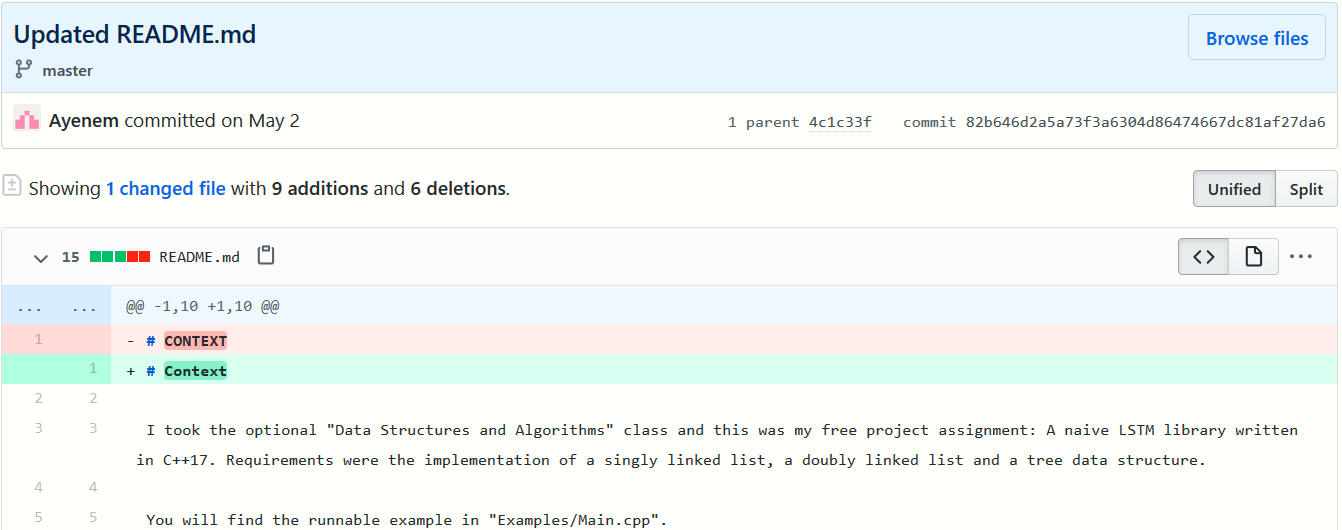
\includegraphics[width=1\textwidth, center]{README_Update}

\subsection{Utilisation}
\subsubsection{Créer un compte}
\begin{enumerate}
  \item Allez sur \url{https://github.com/} et cliquez \textit{"Sign up for GitHub"} 
  
\includegraphics[width=0.3\textwidth, left]{Signup}
  \pagebreak
  \item Remplissez les champs avec vos informations\\\\
  \includegraphics[width=0.38\textwidth, center]{Create_Account}
  
  \item (Optionnel) Répondez aux questions posées par GitHub et validez le tout à la fin.
  
  \item Consultez votre courriel et cliquez sur le bouton \textit{"Verify email address"}.\\
  
\includegraphics[width=0.5\textwidth, center]{Verification}
  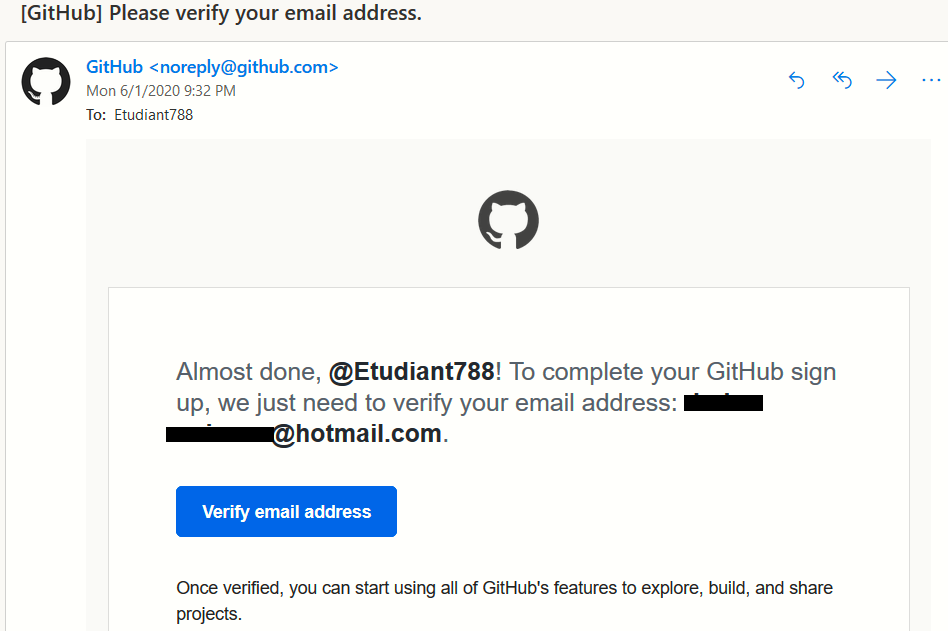
\includegraphics[width=0.4\textwidth, center]{Verification_Email}.
    
  \pagebreak      
  \item À la page \textit{"What do you want to do first?"}, cliquez sur \textit{"Skip this for now"} tout en bas.\\
  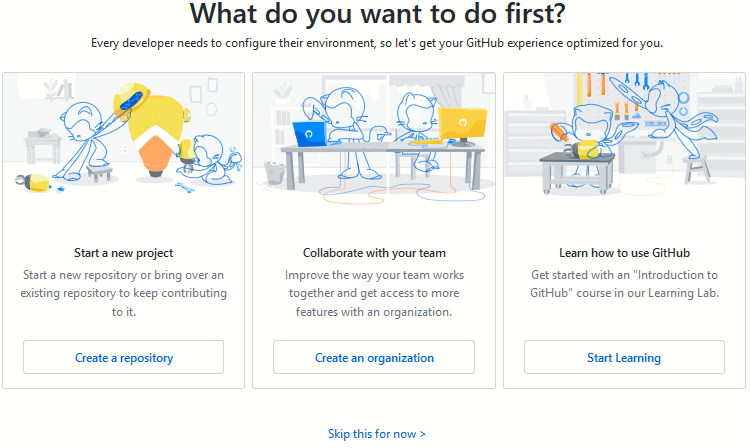
\includegraphics[width=0.58\textwidth, center]{After_Signup}
  
\end{enumerate}

\subsubsection{Créer un dépôt distant sur GitHub}

\begin{enumerate}

  \item Sur la page d'accueil, en haut à gauche, cliquez sur "Create Repository".
  \includegraphics[width=0.15\textwidth, left]{Create_repo}
  
  \item Donnez un nom et une description à votre dépôt. Ne cochez pas la case "\textit{Initialize this repository with a README}". On veut garder le dépôt vide pour pouvoir proprement y importer notre dépôt local plus tard.\\\\
    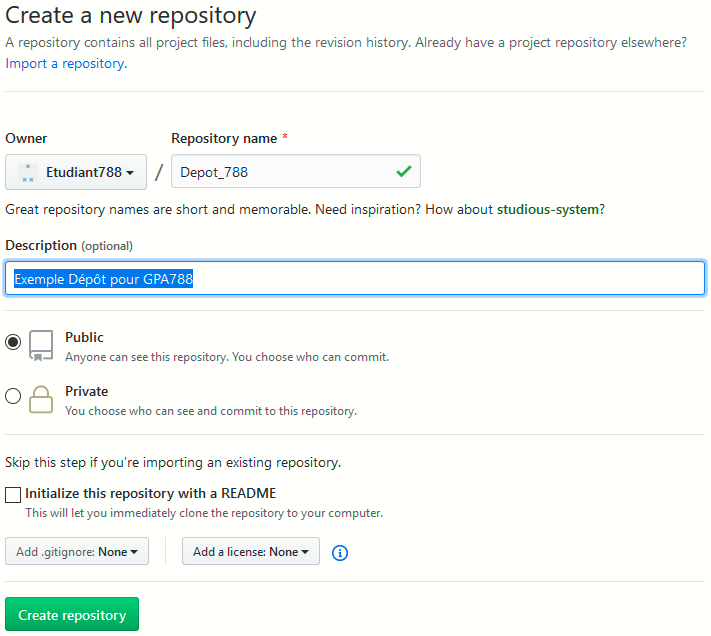
\includegraphics[width=0.6\textwidth, center]{New_Repo}
  
  \pagebreak  
  \item Votre dépôt est créé !\\\\
  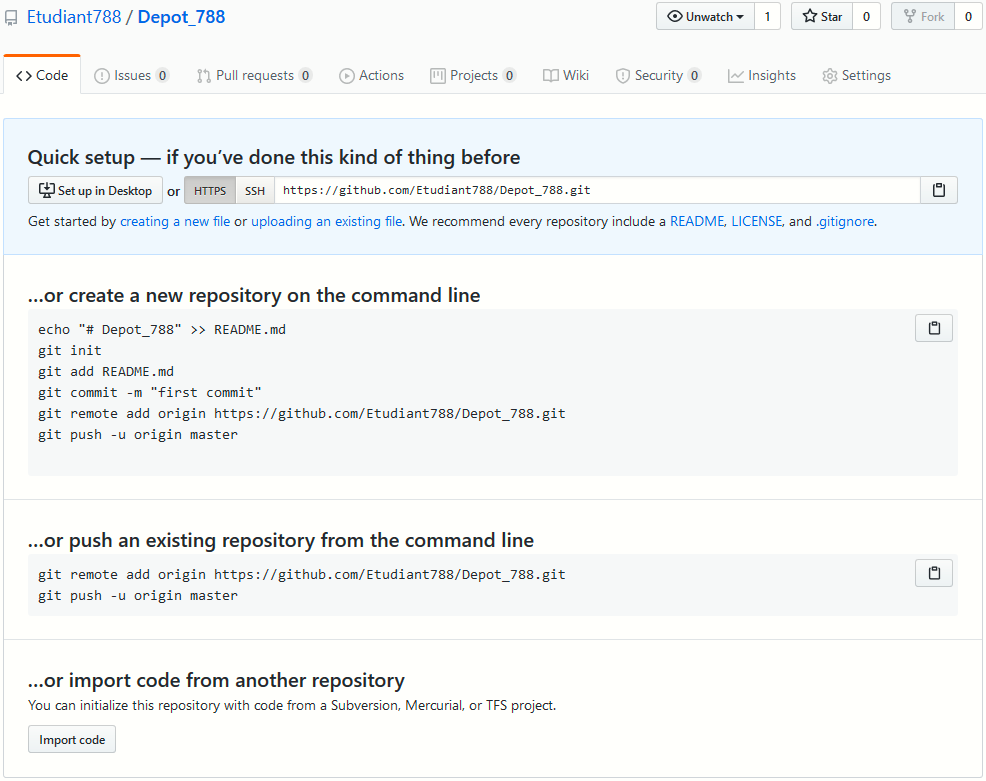
\includegraphics[width=0.85\textwidth, center]{Created_Repo}
  
\end{enumerate}

\begin{flushleft}
GitHub vous propose une liste d'instructions pour associer votre dépôt \textit{GitHub} à votre dépôt local. Ces instructions sont à exécuter sur l'interface de ligne de commande de \textit{Git}.
\end{flushleft}

\begin{center}\section{Git}\end{center}
\subsection{Présentation}
\textit{Git} est le système de contrôle de version utilisé par le service d'hébergement \textit{GitHub}. L'utilisateur doit pouvoir consulter ou manipuler un dépôt distant à partir de sa machine; \textit{Git} fournit cette possibilité à travers une interface de ligne de commande, ou plus rarement, une interface graphique.\\\\

\subsection{Utilisation}
\subsubsection{Installer Git}
\begin{enumerate}
  \item On a besoin d'associer notre dépôt local -le dossier où est notre projet- au dépôt de GitHub. Il est donc temps d'installer l'interface de ligne de commande \textbf{Git}. Pour ce faire, allez sur \url{https://git-scm.com/downloads} et installez la version appropriée à votre OS.
  
  \item Ouvrez l'exécutable téléchargé et suivez les étapes d'installation. Sur Windows, assurez-vous que les cases \textbf{Windows Explorer Integration \& Git Bash Here} sont cochées. Normalement, elles le sont par défaut.\\
  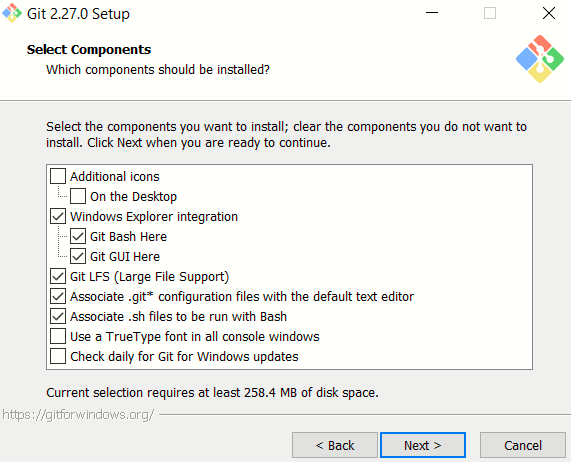
\includegraphics[width=0.55\textwidth, center]{WinExplorer_Integration}
  
  \item Dans ce tutoriel, on privilégie \textbf{Vim} comme éditeur de texte pour Git.\\
  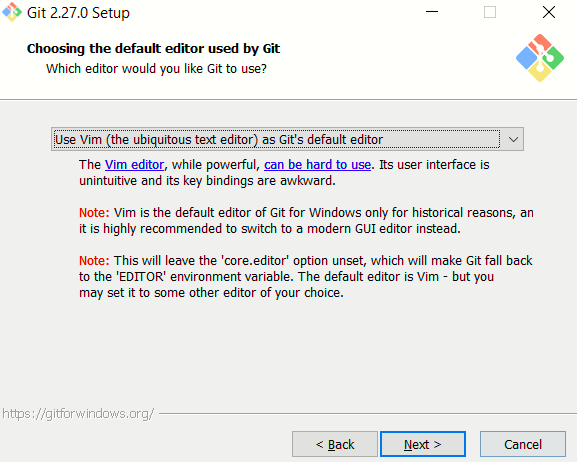
\includegraphics[width=0.55\textwidth, center]{Vim_Choice}
  
  \item Vous pouvez gardez l'option \textbf{Git from the command line and also from 3rd-party software}. Ça offre plus de flexibilité en terme d'accès aux commandes Git par le CLI de Windows ou Powershell, mais ce tutoriel utilisera exclusivement l'interface \textit{Git Bash}.\\\\
  
  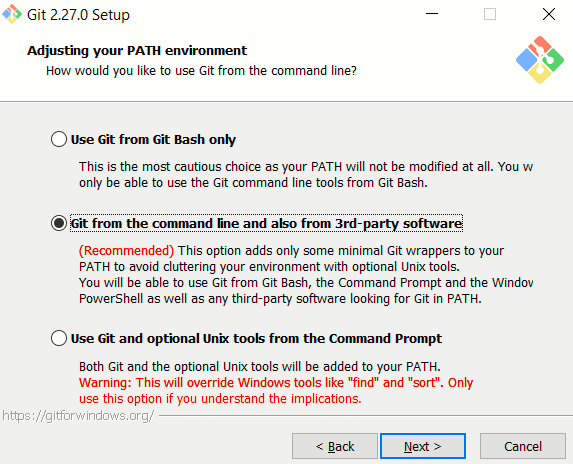
\includegraphics[width=0.55\textwidth, center]{Git_CLI_Choice}
  
  \item Gardez les options par défaut pour la suite de l'installation:
    
    \begin{itemize}
        \item \textbf{Use the OpenSSL library.} Vu qu'on n'est pas en contexte de serveurs distribués.
        
        \item Gestion des conversions CRLF-LF (\textit{Carriage Return Line Feed}) pour la compatibilité multi-plateforme des formats de retour de ligne pour les fichiers texte:\\
        \underline{Pour Windows:} \textbf{Checkout Windows-style, commit Unix-style line endings.}\\
        \underline{Pour Unix:} \textbf{Checkout as-is, commit Unix-style line endings.}
        
        \item \textbf{Use MinTTY (the default terminal of MYSYS2)}. Émulateur du terminal avec plusieurs avantages par rapport au \textit{Windows default console window} (cmd.exe); format Unicode (affichage de caractères non-ASCII), redimensionnabilité de la fenêtre, facilité de selection et de parcours (\textit{scrolling})...etc.

        \item \textbf{\textbf{Default (fast-forward or merge)}}. Comportement standard de la commande \textit{git pull}. Garder ce standard facilitera les recherches de définition ou résolution sur le web.
        
        \item Gardez l'état par défaut des options pour toutes les étapes suivantes jusqu'au \textit{Install}.
    \end{itemize}
\end{enumerate}

\subsubsection{Associer un projet à GitHub}

\begin{enumerate}
    \item Allez au dossier local de votre projet, et cliquez-droit pour accéder à l'option  \textit{Git Bash Here}. Pour les utilisateurs de Linux, vous pouvez juste ouvrir Git et cd vers votre projet.\\
    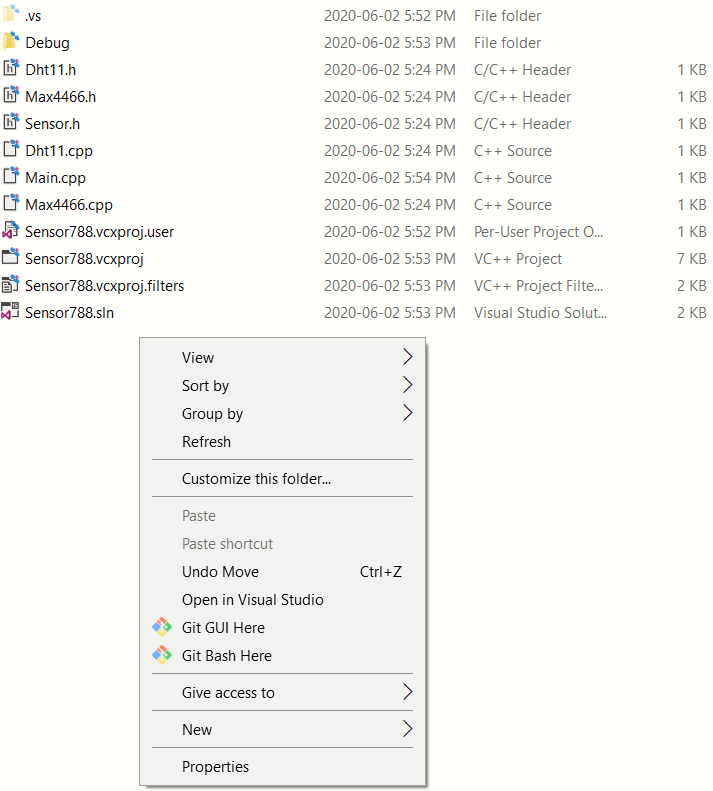
\includegraphics[width=0.45\textwidth, center]{Git_Bash_Here}
    
    \item Tapez les commandes suivantes dans le terminal de Git.
    \begin{itemize}
        \item \textbf{git init} : Votre dépôt local pourra maintenant être considéré comme dépôt de Git.
        
        \item \textbf{git config --global user.email "adresse courriel"}: Associe le dépôt local avec l'adresse courriel utilisée pour votre compte GitHub
        
        \item \textbf{git config --global user.name "Nom utilisateur"}: Associe le dépôt local avec le nom d'utilisateur utilisé pour votre compte GitHub
        
        \item \textbf{git add .} ou \textbf{git add --all}: Ajoute les fichiers au dépôt local.
        
        \item \textbf{git commit -m "First Commit"} : Enregistre les changements traqués et les prépare pour un \textit{push} au dépôt GitHub.
    
        \item \textbf{git remote add origin} \textcolor{Blue}{adresse\_URL\_du\_dépôt.git}\\\\
        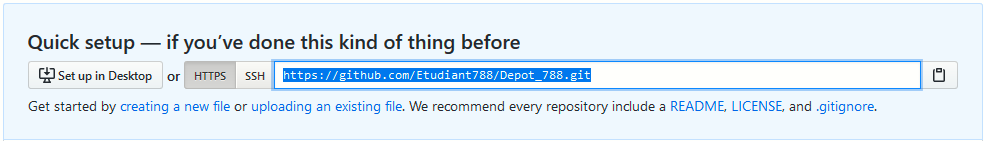
\includegraphics[width=0.9\textwidth, center]{Git_URL}
        Si vous n'avez plus accès au \textit{Quick setup} pour l'adresse, utilisez \textbf{"Clone or download"} sur la page du dépôt:\\
        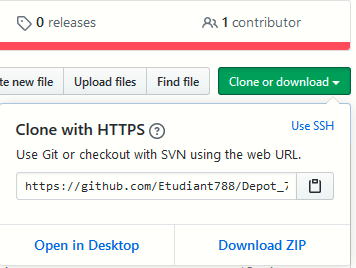
\includegraphics[width=0.37\textwidth, center]{Clone_Download}
    
        \item \textbf{git push -u origin master} : Les changements du dépôt local sont poussés vers le dépôt distant (GitHub).
    \end{itemize}
    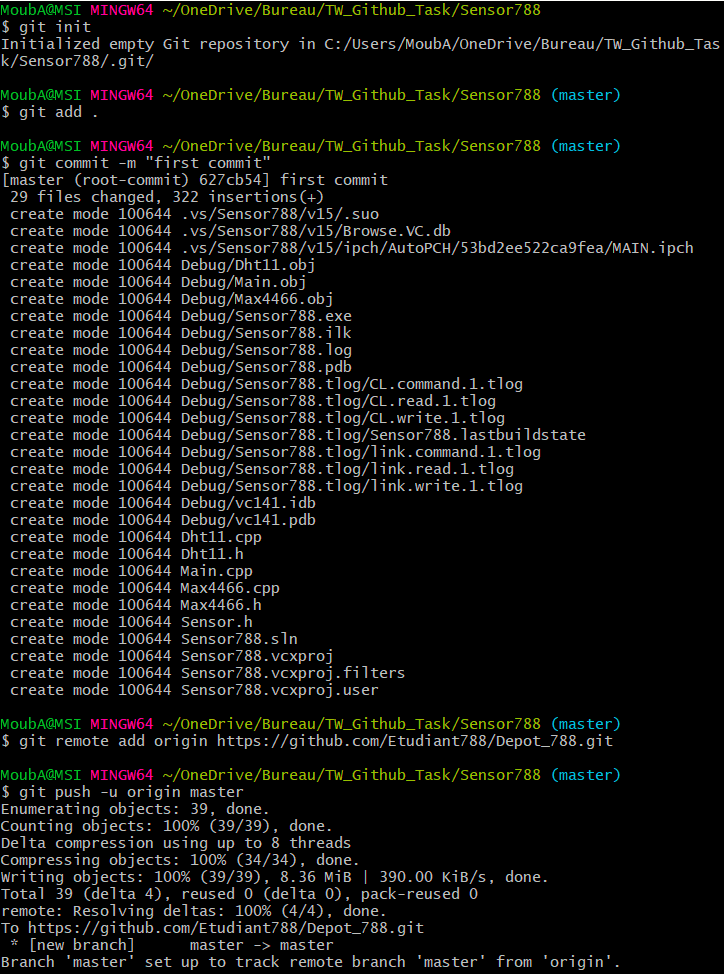
\includegraphics[width=0.6\textwidth, center]{Git_Terminal}
    
    \item \textcolor{Red}{\textbf{Voici la routine à exécuter lorsque vous voudrez synchroniser les changements du dépôt local avec le dépôt distant de GitHub:}}
    \begin{lstlisting}[language=bash]
        git add .
        git commit -m "Message"
        git push
    \end{lstlisting}
\end{enumerate}

\begin{center}\section{Travail Collaboratif}\end{center}

\subsection{Mise en place}
Dans cet exemple, le compte \textit{propriétaire} sera \textbf{Etudiant788}, et le \textit{compte collaborateur} sera \textbf{Ayenem}.
Le propriétaire doit donner accès au collaborateur. Sur GitHub: Settings $\rightarrow$ Manage access $\rightarrow$ \textbf{Invite a collaborator}.\\\\
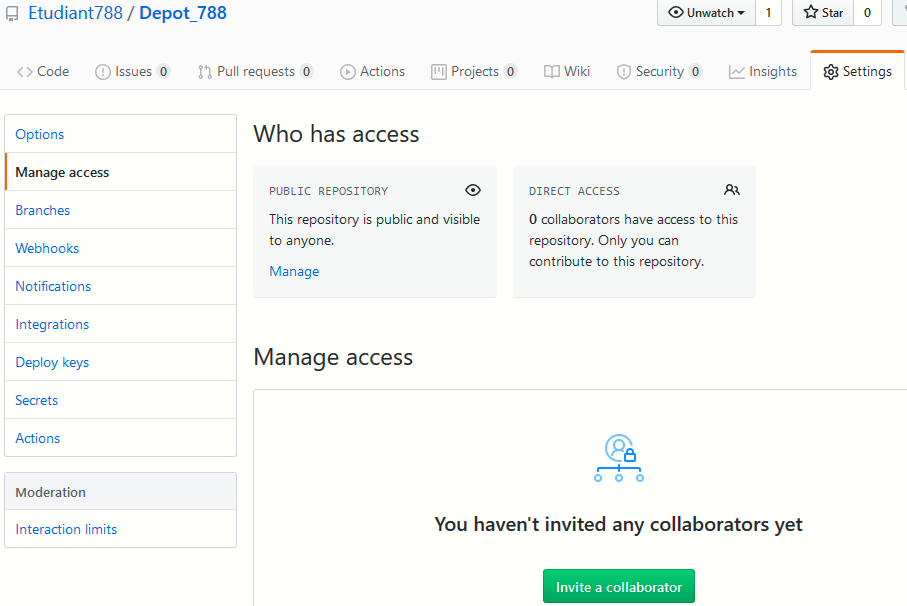
\includegraphics[width=0.55\textwidth, center]{Invite_Collaborator}

\begin{flushleft}
Le collaborateur devrait recevoir un courriel avec un bouton \textbf{View Invitation}. Suivre le lien puis accepter l'invitation.\\
\end{flushleft}
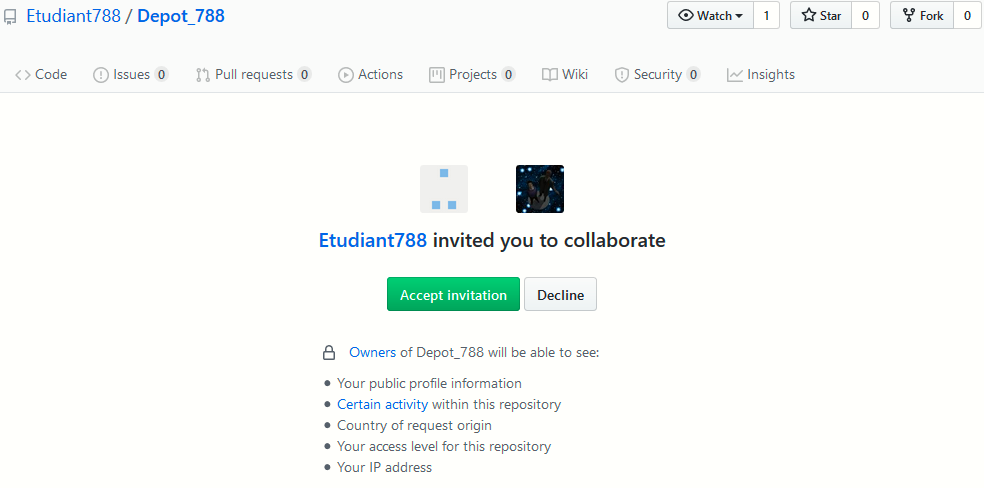
\includegraphics[width=0.55\textwidth, center]{Collab_Invite}

\begin{flushleft}
Le collaborateur a maintenant accès en écriture et publication (\textit{push access}) au dépôt du propriétaire:\\
\end{flushleft}
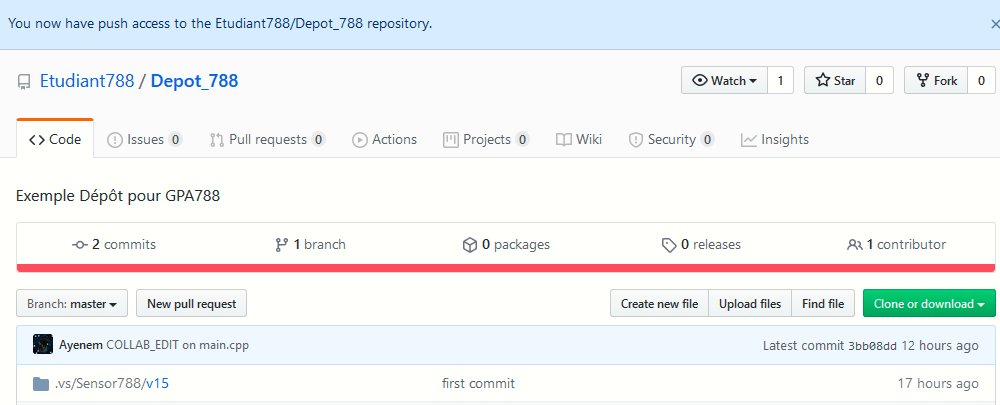
\includegraphics[width=0.8\textwidth, center]{Collab_Access}

\begin{flushleft}
Le collaborateur doit cloner le dépôt sur sa machine, pour ce faire, il doit ouvrir le terminal Git Bash dans le dossier où il souhaite télécharger le projet, et exécuter:
\end{flushleft}

\begin{center}
    \textbf{git clone} \textit{adresse du dépôt du propriétaire}\\
\end{center}

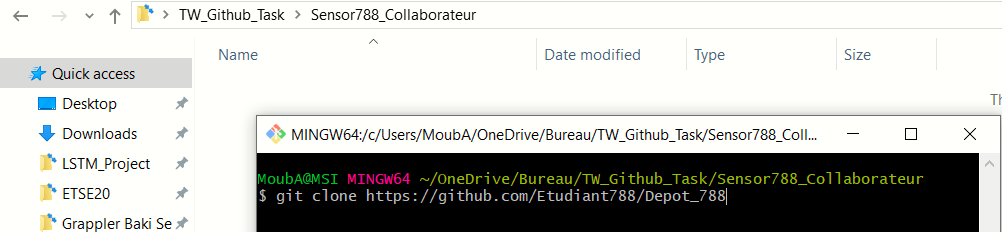
\includegraphics[width=0.7\textwidth, center]{Git_Clone}

\begin{flushleft}
Le collaborateur peut maintenant effectuer des changements sur son clone local du dépôt, puis exécuter la routine (à partir du répertoire des fichiers à modifier, contenant le dossier caché \textit{.git}):
\end{flushleft}
\begin{lstlisting}[language=bash]
    git add .
    git commit -m "Message"
    git push
\end{lstlisting}

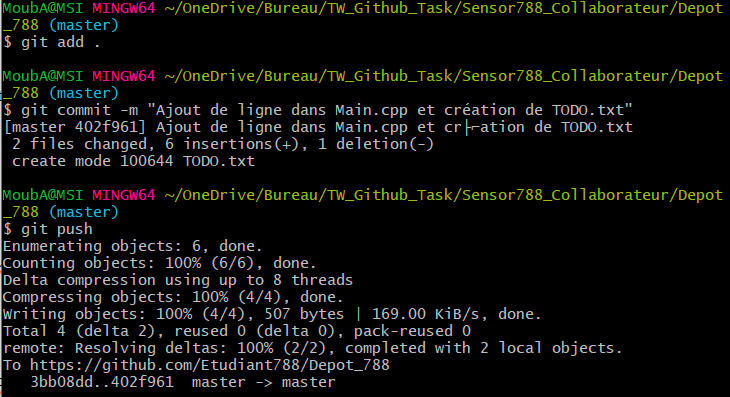
\includegraphics[width=0.55\textwidth, center]{Collab_Push}

\pagebreak
\begin{flushleft}
Le propriétaire peut actualiser la page de son dépôt et remarquer les changements publiés par le collaborateur:
\end{flushleft}
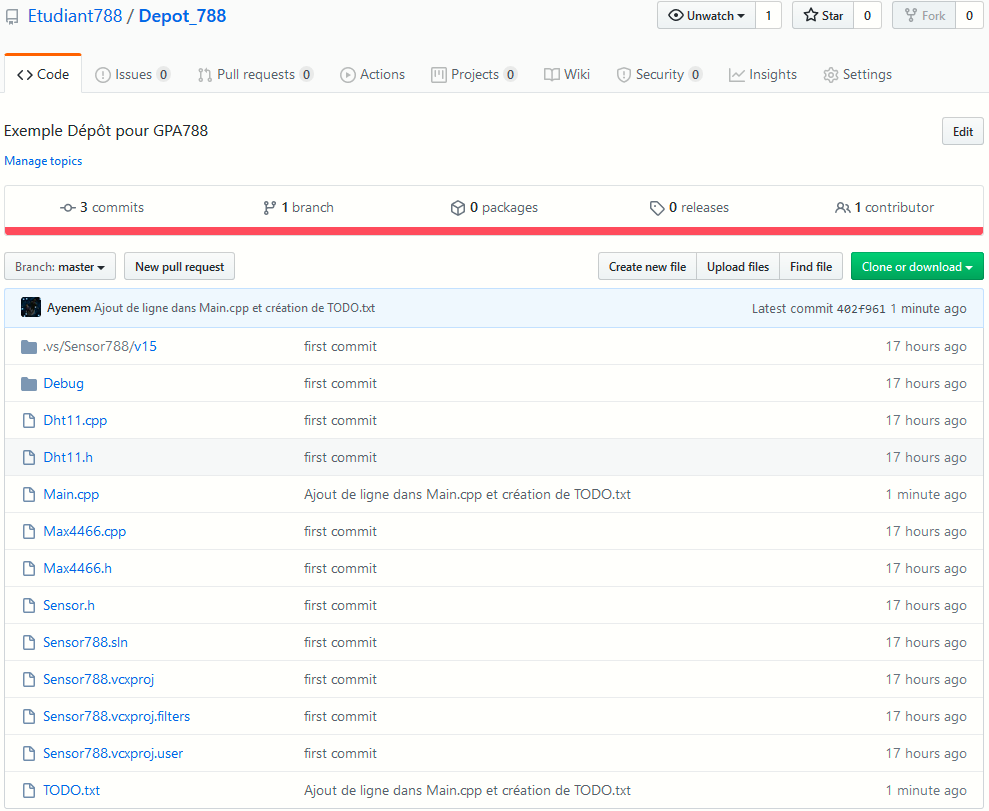
\includegraphics[width=0.69\textwidth, center]{Proprio_Perspective}

\begin{flushleft}
Il est également possible d'afficher un différentiel des changements effectués sur le dépôt. Pour ce faire, il suffit de cliquer sur le message du \textit{commit} accompagnant le fichier:
\end{flushleft}
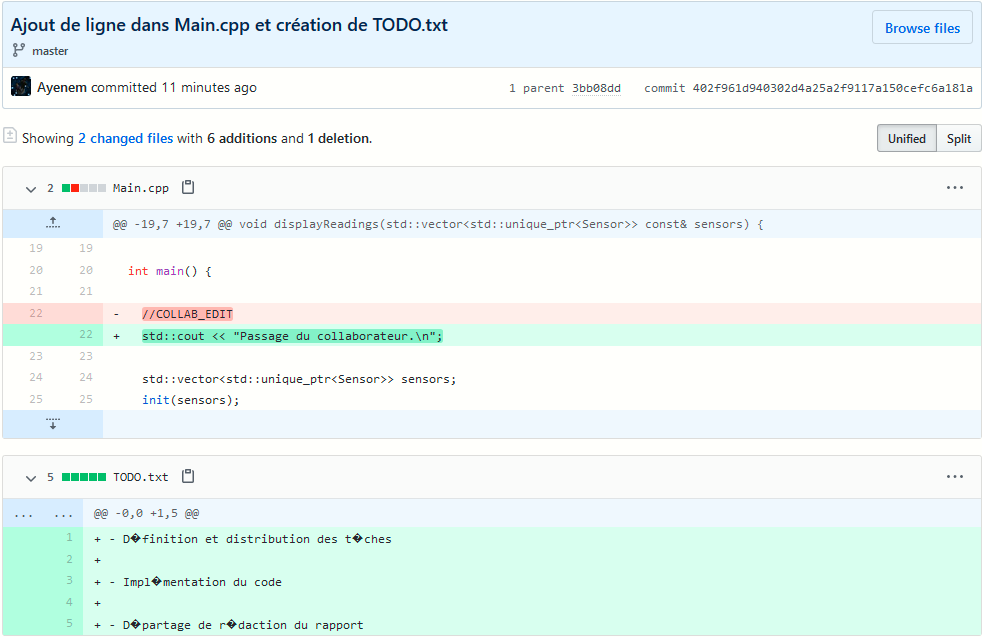
\includegraphics[width=0.69\textwidth, center]{GitHub_Diff}

\subsection{Méthodologie collaborative de base}

Il est fortement conseillé de s'assurer d'être à jour sur le dépôt sur lequel vous collaborez. Pour ce faire, \textcolor{Red}{\textbf{effectuez toujours un git pull avant de faire des modifications}}. Le flux de travail de base ressemble à ceci:
\begin{enumerate}
    \item Mettez à jour votre dépôt local avec \textbf{git pull origin master}
    \item Effectuez vos modifications et ajoutez-les avec \textbf{git add --all} ou \textbf{git add .}
    \item Enregistrez vos modifications avec \textbf{git commit -m "Message décrivant le changement"}
    \item Poussez les modifications au dépôt GitHub avec \textbf{git push}.
\end{enumerate}
Il est préférable d'effectuer plusieurs \textit{commit} avec des petits changements, plutôt qu'un seul avec plusieurs changements. Les petits \textit{commit} sont plus faciles à lire et réviser.

\begin{center}\section{Ressources utiles}\end{center}
\begin{itemize}
  \item Documentation officielle de git: \url{https://git-scm.com/docs/git-help}
  
  \item Google et stackoverflow.com sont vos amis
  
  \item Visualisation des concepts de git: \url{https://onlywei.github.io/explain-git-with-d3/}
  
  \item Pour tester l'aperçu du format markdown (pour README.md) en ligne: \url{https://dillinger.io/}
  
  \item Si comme moi vous ne supportez pas quand tous les pixels non-pertinents sont activés et stimulent les yeux inutilement pour une grande partie de l'écran, voici des add-ons pour \textit{GitHub Dark Theme}:\\
    \underline{Pour Mozilla Firefox:}\\
    \url{https://addons.mozilla.org/en-CA/firefox/addon/github-dark-theme/}\\
    \underline{Pour Google Chrome:}\\
    \url{https://tinyurl.com/githubDarkThemeForChrome}\\
    \underline{Pour Internet Exp...}\\
    
\includegraphics[width=0.6\textwidth, center]{Cool_Github_Logo}
\end{itemize}

\end{document}
